\section{目的}
依據 \textit{AIC Lab.pdf} PDF 31--40 頁，完成兩種 diode-load CS、current-source-load CS 及 N/P source follower，逐一核對尺寸、偏壓、輸出阻抗、增益與頻寬。使用由使用者另行提供的模型庫，供應電壓為 1.0 V。這是本次教學適配條件，並非模型額定電壓的認證；講義原製程的 3.3 V 圖表與數字不直接當作通過門檻。程式依講義拓樸重寫，原始程式僅作尺寸與缺漏的參考。

\section{Spec 對照}
S 表示實際模擬；D 表示推導與討論。舊製程增益表為比較背景，不是本次模型的保證值。
\small\begin{longtable}{p{.46\linewidth}p{.30\linewidth}p{.15\linewidth}}\toprule
要求與 PDF 頁碼 & 對應 deck／檢查 & 狀態 \\ \midrule\endhead
PMOS diode-load CS，W=100/200/300（31--32） & D01; DC/AC/Rout & S+D \\
NMOS diode-load CS，W=150/200/300（33--34） & D02; DC/AC/Rout & S+D \\
兩種 diode load 的增益、GB 與優缺點（34） & D01--02; derivatives & S+D \\
Current-load CS、等 W/L 尺度、鏡像準確度（35--37） & D03/C0,C5,C6 & S+D \\
NMOS/PMOS source follower 比較（38--39） & D04; gain/BW & S+D \\
CS W=10/18/26 與 Iref=100/166/333（39--40） & D03/C0--C4 & S+D \\
低電流適配與時域檢查 & D03/C7--C9, D05 & S; adapted \\
\bottomrule\end{longtable}\normalsize


\section{電路與設計推導}
\[
A_{v,P}\simeq-\frac{g_{m1}}{g_{ds1}+g_{m2}+g_{ds2}},\quad
A_{v,N}\simeq-\frac{g_{m1}}{g_{ds1}+g_{m2}+g_{mb2}+g_{ds2}}.
\]
\[
A_{v,CS}\simeq-\frac{g_{mn}}{g_{dsn}+g_{dsp}},\qquad
A_{v,SF}\simeq\frac{g_m}{g_m+g_{mb}+g_{ds,F}+g_{ds,load}}.
\]表中的 $g_m$ estimate 使用該案例實際 \texttt{.op} 導數，並非套用未確認的遷移率。$R_o$ 由 \texttt{.tf} 的小訊號輸出電阻取得；電容在 DC 開路。$GB=|A_v(1\,\mathrm{Hz})|f_{3dB}$ 與實際 unity crossing 分開保存，對多極點電路不強行當成同一量。

D01/D02 保留講義負載 $W/L=2/1\,\mu$m、$C_L=10$ pF，主動元件依題目掃寬度，全部 $L=1\,\mu$m。PDF 33 將 NMOS body 說成接 VDD 與一般 P-substrate 結構不符；本次接地並保留 $g_{mb}$。原碼缺少這兩種 diode-load 拓樸，本次補齊。

D03/C0--C4 的 $(W_n,W_p,L,I_{ref})$ 依序為 $(10,30,1,100)$、$(18,30,1,100)$、$(26,30,1,100)$、$(10,30,1,166)$、$(10,30,1,333)$，尺寸單位 $\mu$m、電流單位 $\mu$A。C5/C6 將 C0 的所有 W、L 一起乘 3/5，保持 W/L；C7--C9 為 10 $\mu$A，$W_n=10/18/26\,\mu$m 的另列適配。每個 CS 的輸入偏壓由 DC 曲線和局部導數校準至約 0.5 V 輸出，沒有在待測電路加入伺服放大器。

D04 的 N/P follower 皆用 $W/L=30/1\,\mu$m、$C_L=10$ pF；閘極分別為 0.9/0.1 V，電流依 C0--C3 為 100/10/166/333 $\mu$A。不同分析使用一致電路，修正原碼跨 DC/AC/transient 尺寸不一致及超出供應的輸入。

\section{模擬設定}
使用 PrimeSim HSPICE S-2021.09 win64，基本溫度 27 $^\circ$C，\texttt{runlvl=5}、\texttt{accurate}，輸出 \texttt{.op/.print/.measure}。每個 \texttt{.alter} 先重設完整基準參數與溫度，防止前一案例殘留。實際工作已完成，未出現 error 或 failed 量測；模型仍有被抑制的警告訊息，因此不宣稱完全沒有 warning。公開 netlist 不含模型路徑，以下註解標示本機執行前必須設定的模型入口；模型檔與設定只保留本機：
\begin{verbatim}
* MODEL_SETUP_REQUIRED
\end{verbatim}
CSV 與數值摘要位於該 lab 的 \texttt{results/}；所有圖均由真實列印數據重繪，不是波形軟體畫面截圖。\texttt{manifest.json} 提供 spec 對照與案例定義。五份 deck 共 23 個案例。CS DC 掃描為 0--1 V、1 mV 步距；AC 為 1 Hz--10 GHz、60 points/decade，輸入 AC=1 V。Follower 的 DC 掃描只改 NMOS 輸入，PMOS 維持 0.1 V；其 N/P AC 電路各自獨立，避免把互相反相的輸入當同一增益。D05 為 1 kHz、5 ms，最後一週期量峰對峰；CS 振幅 0.1/1/3 mV，follower 振幅 10 mV。

\section{結果與規格檢查}
\begin{center}\small\begin{tabular}{lrrrrrr}\toprule
Case & $V_{in}$ (V) & $|A_v|$ & $g_m$ estimate & $R_o$ (k$\Omega$) & $f_{3dB}$ (MHz) & Sat. \\ \midrule
D01/C0 & 0.21622 & 2.35 & 2.35 & 43.07 & 0.366 & Y \\
D01/C1 & 0.18785 & 2.41 & 2.41 & 43.05 & 0.363 & Y \\
D01/C2 & 0.17159 & 2.44 & 2.45 & 43.04 & 0.360 & Y \\
D02/C0 & 0.19697 & 1.11 & 1.11 & 21.35 & 0.736 & Y \\
D02/C1 & 0.18532 & 1.13 & 1.13 & 21.35 & 0.733 & Y \\
D02/C2 & 0.16909 & 1.14 & 1.14 & 21.35 & 0.727 & Y \\
D03/C0 & 0.55243 & 124.30 & 124.34 & 126.10 & 0.125 & Y \\
D03/C1 & 0.49981 & 156.65 & 156.69 & 125.30 & 0.126 & Y \\
D03/C2 & 0.47225 & 174.09 & 174.13 & 123.60 & 0.128 & Y \\
D03/C3 & 0.60983 & 69.37 & 69.39 & 54.73 & 0.289 & Y \\
D03/C4 & 0.71517 & 11.10 & 11.10 & 6.68 & 2.363 & N \\
D03/C5 & 0.55481 & 179.14 & 179.92 & 181.20 & 0.086 & Y \\
D03/C6 & 0.55539 & 201.82 & 204.63 & 204.10 & 0.075 & Y \\
D03/C7 & 0.39126 & 227.10 & 227.14 & 1208.00 & 0.013 & Y \\
D03/C8 & 0.36092 & 233.00 & 233.05 & 1159.00 & 0.014 & Y \\
D03/C9 & 0.34283 & 234.85 & 234.92 & 1133.00 & 0.014 & Y \\
\bottomrule\end{tabular}\end{center}
Sat.=Y 僅表示此名義操作點的所有元件滿足 $|V_{DS}|\ge|V_{DSAT}|$；不代表強反轉或整段輸出擺幅皆有效。Subthreshold 標記保留在 \texttt{operating\_points.csv}。例如 diode-load CS 在本次偏壓常進入弱反轉，因此不應用強反轉的 $\sqrt{W}$ 比例強行要求增益。

\begin{figure}[htbp]\centering
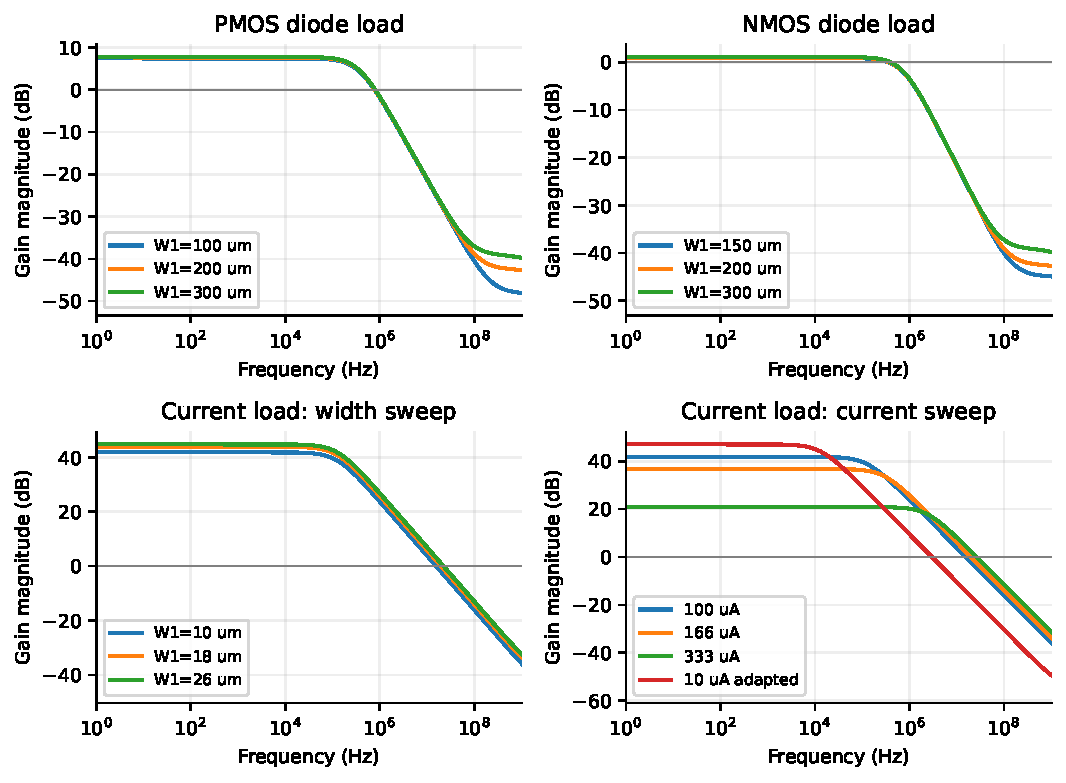
\includegraphics[width=\linewidth]{figures/gain_comparison.pdf}
\caption{兩種 diode load 及 current-source load 的實際 Bode 曲線。電流與幾何比較均保留各自操作點。}
\end{figure}
\begin{center}\small\begin{tabular}{lrrrr}\toprule
$I_{ref}$ ($\mu$A) & $A_n$ & $A_p$ & $f_n$ (MHz) & $f_p$ (MHz) \\ \midrule
100 & 0.8260 & 0.6855 & 27.032 & 12.355 \\
10 & 0.8337 & 0.8503 & 3.992 & 2.856 \\
166 & 0.8217 & 0.5344 & 38.088 & 17.654 \\
333 & 0.8079 & 0.4060 & 57.736 & 25.284 \\
\bottomrule\end{tabular}\end{center}
\begin{center}\small\begin{tabular}{lrrr}\toprule
Input amplitude (mV) & CS output p-p (V) & Effective $|A_v|$ & Follower p-p (V) \\ \midrule
0.1 & 0.04521 & 226.04 & 0.01667 \\
1 & 0.42794 & 213.97 & 0.01667 \\
3 & 0.74588 & 124.31 & 0.01667 \\
\bottomrule\end{tabular}\end{center}
\begin{center}\small\begin{tabular}{lrr}\toprule
D03 case & Mirror error (\%) & $GB$ (MHz) \\ \midrule
0 & -0.492 & 15.594 \\
1 & -0.492 & 19.764 \\
2 & -0.492 & 22.256 \\
3 & -0.968 & 20.051 \\
4 & -3.926 & 26.230 \\
5 & -0.337 & 15.450 \\
6 & -0.292 & 15.224 \\
7 & 0.392 & 2.976 \\
8 & 0.392 & 3.180 \\
9 & 0.392 & 3.278 \\
\bottomrule\end{tabular}\end{center}
D03 的鏡像誤差定義為 $(|I_{MP}|/|I_{MREF}|-1)\times100\%$。333 $\mu$A 案例仍保留，但較小的參考端裕量與元件工作區會限制其增益；不得只比較寬度而忽略實際偏壓。D05 的 0.1 mV 輸入接近小訊號結果，較大振幅的有效增益下降，顯示 DC 轉移曲線彎曲。
\begin{figure}[htbp]\centering
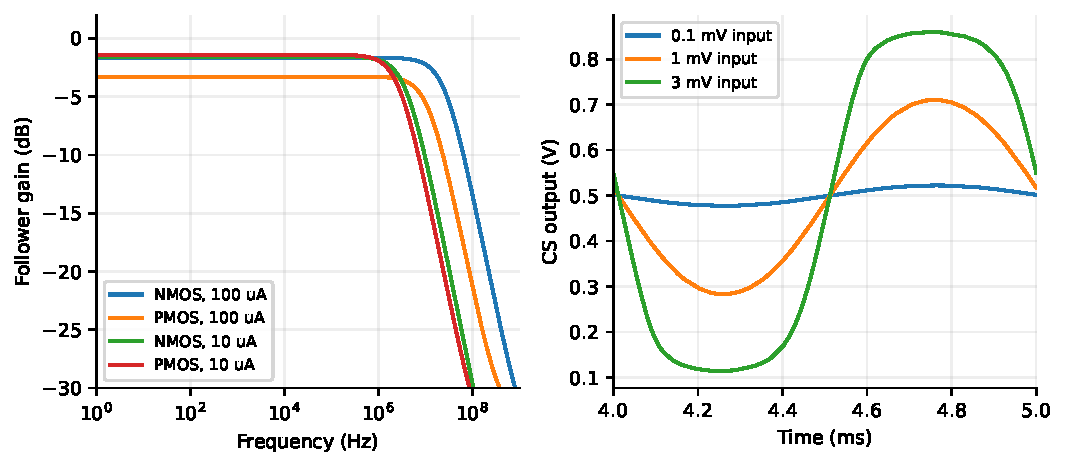
\includegraphics[width=\linewidth]{figures/followers_transient.pdf}
\caption{N/P follower 的頻率響應與 CS 的振幅比較。右圖為最後一個 1 kHz 週期的實際輸出。}
\end{figure}


\section{討論}
在相同負載尺寸下，PMOS diode load 因遷移率、偏壓與缺少相同的 NMOS source-body 項，可能具有較小負載跨導並得到較大 CS 增益；但這是有條件的比較，不是每個製程和偏壓都必然成立。Diode load 易偏壓、元件少且輸出阻抗低，代價是增益較小及消耗電壓裕量。增大輸入 $g_m$ 或減小有效負載導納可提高增益；增加電流、減少負載電容可改善速度，但同時改變功耗、輸出阻抗與偏壓。

Current-source load 減少 $g_m$ 負載項，提升增益但對電流匹配及輸出工作點更敏感。在固定電流下，增加 W 可提高強反轉 $g_m$，但也增加電容；提高電流使 $g_m$ 與 $g_{ds}$ 同時變動，因此增益不必提高。等 W/L 而拉長 L 可降低通道長度調變、改善鏡像準確度，但面積與寄生電容增加。

Source follower 的增益被 body effect 與有限負載導納拉低。100 $\mu$A 時 NMOS 較接近 1，但 10 $\mu$A 時本次 PMOS 增益約 0.8503，反而高於 NMOS 約 0.8337；不能把講義舊圖的 N-type 優勢當成普遍定理。

\section{結論}
講義的主要拓樸、寬度／電流／等 W/L 尺度變化均已實際測試，且補上原碼缺少的 diode load。增益、頻寬與非線性結果適用於各自列出的偏壓；未將原製程數字或全 PVT 成功混為已驗證成果。

